\chapter{心脏与血液}\label{ch:g4:heart-and-blood}

用两根手指（不要用拇指）按在手腕内侧，
拇指根部下方，静静等待。你会感觉到一下轻微而平稳的
跳动，一下接一下，大约每秒一次。这种跳动就是你的
\omterm{def:g4:heart-and-blood:heart}{心脏}在工作，在手腕上就能感觉到。它从你出生之前
就一直在跳动，是身体运送系统的
发动机。

\section{血液：身体的运送系统}

\begin{proposition}[血液携带的物质]\label{prop:g4:heart-and-blood:carries}
\emph{血液}\index{血液}是一种液体，它能到达身体的每个角落，
是身体的“运输工”：
\begin{itemize}
  \item 从\omterm{def:g4:journey-of-food:tract}{小肠}中收集
        \emph{\omterm{def:g4:journey-of-food:digestion}{营养物质}}（\cref{prop:g4:journey-of-food:absorb}）；
  \item 从肺中收集\emph{氧气}
        （\cref{prop:g4:breathing:exchange}）；
  \item 把两者输送到身体的各个部分——\omterm{def:g3:bones-and-muscles:muscle}{肌肉}、
        脑、骨和\omterm{def:g1:the-five-senses:sense}{皮肤}；
  \item 在返回途中带走废物，把
        二氧化碳运到肺部，再呼出体外。
\end{itemize}
\end{proposition}
\admitted

\begin{example}[一次运送的过程]\label{ex:g4:heart-and-blood:round}
跟踪一滴\omterm{prop:g4:journey-of-food:absorb}{血液}的路线：在肺中，它变成鲜红色，
载满氧气；\omterm{def:g4:heart-and-blood:heart}{心脏}将其送出；在奔跑的腿部
\omterm{def:g3:bones-and-muscles:muscle}{肌肉}中，它交出氧气和\omterm{def:g4:journey-of-food:digestion}{营养物质}，接收二氧化碳，
颜色变暗；回到\omterm{def:g4:heart-and-blood:heart}{心脏}后，它被送往
肺部卸下二氧化碳、重新装载氧气，然后再次出发。一次完整的循环
用时远不到一分钟。
\end{example}

\begin{definition}[血管]\label{def:g4:heart-and-blood:vessels}
\omterm{prop:g4:journey-of-food:absorb}{血液}在称为
\emph{血管}\index{血管}的管道中流动：离开\omterm{def:g4:heart-and-blood:heart}{心脏}和流回\omterm{def:g4:heart-and-blood:heart}{心脏}的是较粗的血管，它们
逐级\omterm{def:g1:plants-around-us:tree}{分支}、越来越细——最细的
毛细血管像发丝一样穿行于身体各部分之间，
在那里完成物质交换。把一个人全身的血管首尾相连，
长度可达数万千米。
\end{definition}

\begin{remark}[看见血管]\label{rem:g4:heart-and-blood:see}
看看你手腕的内侧：\omterm{def:g1:the-five-senses:sense}{皮肤}下方有一些青色的细线
——那是正在回流\omterm{def:g4:heart-and-blood:heart}{心脏}的\omterm{def:g4:heart-and-blood:vessels}{血管}。
擦伤的膝盖则显示了\omterm{def:g4:heart-and-blood:vessels}{血管}网络的另一端：即使
最细小的伤口也会渗血，因为最细的\omterm{def:g4:heart-and-blood:vessels}{血管}
遍布全身。
\end{remark}

\section{心脏：泵}

\begin{definition}[心脏]\label{def:g4:heart-and-blood:heart}
\emph{心脏}\index{心脏}是一个空心的\omterm{def:g3:bones-and-muscles:muscle}{肌肉}器官，大小约与
主人的拳头相当，位于胸腔中部、\omterm{def:g3:bones-and-muscles:skeleton}{肋骨}之后。
心脏通过收缩——即一次\emph{搏动}\index{心跳}——
推动\omterm{prop:g4:journey-of-food:absorb}{血液}在\omterm{def:g4:heart-and-blood:vessels}{血管}中流动。心脏分为两侧：
右侧把\omterm{prop:g4:journey-of-food:absorb}{血液}泵往\emph{肺}，使\omterm{prop:g4:journey-of-food:absorb}{血液}装载氧气；
左侧把富含氧气的\omterm{prop:g4:journey-of-food:absorb}{血液}泵往\emph{全
身}。
\end{definition}

\begin{omfigure}
\begin{tikzpicture}[scale=0.95]
  % heart: two chambers schematic
  \draw[thick, fill=omThm!10] (0,0)
    .. controls (-1.5,0.9) and (-1.3,2.3) .. (-0.35,2.3)
    .. controls (-0.05,2.3) and (0.0,2.15) .. (0.0,2.05)
    .. controls (0.0,2.15) and (0.05,2.3) .. (0.35,2.3)
    .. controls (1.3,2.3) and (1.5,0.9) .. (0,0);
  \draw[thick] (0,2.05) -- (0,0.35);
  \node[font=\small, align=center] at (-0.55,1.45) {右侧};
  \node[font=\small, align=center] at (0.55,1.45) {左侧};
  % arrows: right side to lungs
  \draw[->, very thick, omDef] (-0.55,2.3) .. controls (-0.8,3.0)
    .. (-1.9,3.2)
    node[left, font=\small, omDef, align=center] {送往肺部：\\ 装载氧气};
  \draw[->, very thick, omDef!50] (-3.0,2.2) .. controls (-2.0,2.0)
    .. (-1.15,1.6);
  \node[font=\small, omDef!80, align=center, left] at (-3.05,2.2)
    {从身体 \\ 回流};
  % arrows: left side to body
  \draw[->, very thick, omThm] (0.55,2.3) .. controls (0.8,3.0)
    .. (1.9,3.2)
    node[right, font=\small, omThm, align=center] {送往全身：\\ 输送氧气};
  \draw[->, very thick, omThm!50] (3.0,2.2) .. controls (2.0,2.0)
    .. (1.15,1.6);
  \node[font=\small, omThm!80, align=center, right] at (3.05,2.2)
    {从肺部 \\ 回流};
\end{tikzpicture}

{\small \omterm{def:g4:heart-and-blood:heart}{心脏}的两侧：右侧把\omterm{prop:g4:journey-of-food:absorb}{血液}送往
肺部获取氧气；左侧把装载了氧气的\omterm{prop:g4:journey-of-food:absorb}{血液}
送往全身。}
\end{omfigure}

\begin{proposition}[脉搏]\label{prop:g4:heart-and-blood:pulse}
每次\omterm{def:g4:heart-and-blood:heart}{心跳}都会推动一小股\omterm{prop:g4:journey-of-food:absorb}{血液}波沿\omterm{def:g4:heart-and-blood:vessels}{血管}传播；在
手腕或颈部感觉到的这股波动，就是
\emph{脉搏}\index{脉搏}。数\omterm{prop:g4:heart-and-blood:pulse}{脉搏}就是数
\omterm{def:g4:heart-and-blood:heart}{心跳}次数：儿童静止时每分钟约 $80$ 至 $100$ 次，
成人约为 $60$ 至 $80$ 次，运动时则会增加很多。
\end{proposition}
\admitted

\begin{example}[心脏跟上双腿的节奏]\label{ex:g4:heart-and-blood:effort}
跑步时，腿部\omterm{def:g3:bones-and-muscles:muscle}{肌肉}快速消耗\omterm{def:g4:journey-of-food:digestion}{营养物质}和氧气，
运送也必须加快。因此\omterm{def:g4:heart-and-blood:heart}{心脏}跳得\emph{更快}，
也更有力——儿童冲刺时\omterm{prop:g4:heart-and-blood:pulse}{脉搏}可超过 $150$ 次——同时
\omterm{def:g4:breathing:movements}{呼吸}随之加快，以便为\omterm{prop:g4:journey-of-food:absorb}{血液}重新装载氧气
（\cref{ex:g4:breathing:running}）。\omterm{def:g4:heart-and-blood:heart}{心脏}与肺是
同一条供应链的两个环节。
\end{example}

\begin{method}[测量脉搏]\label{met:g4:heart-and-blood:pulse}
\begin{enumerate}
  \item 一只手掌心朝上摊开；用另一只手的两根手指
        按在腕部，就在拇指根部下方——
        千万不要用拇指，它自己也有微弱的\omterm{prop:g4:heart-and-blood:pulse}{脉搏}；
  \item 轻轻按压，直到感觉到一下一下的\omterm{def:g4:heart-and-blood:heart}{搏动}；
  \item 数一分钟内的\omterm{def:g4:heart-and-blood:heart}{搏动}次数（带秒针的钟表会有
        帮助）；
  \item 把次数记下来，并写下身体当时的状态：
        静止、步行，或刚冲刺之后。
\end{enumerate}
\end{method}

\begin{omfigure}
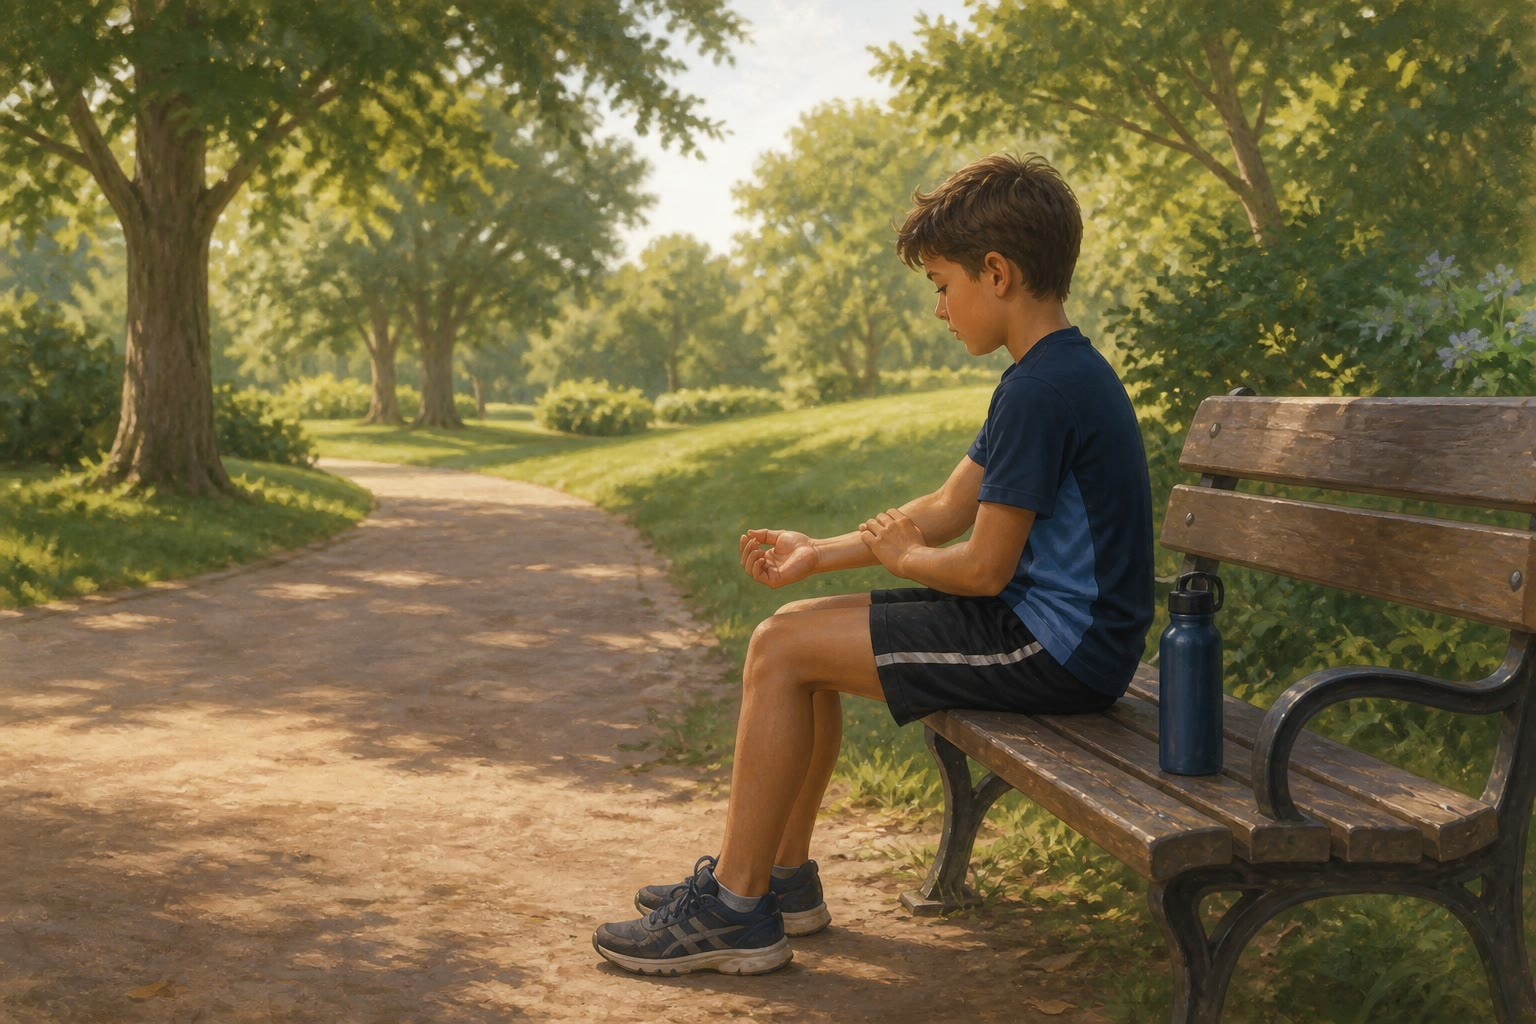
\includegraphics[width=0.58\linewidth]{images/book1/ai/g4-heart-rest.jpg}

{\small 跑步之后：两根手指按在腕部，
远远数着\omterm{def:g4:heart-and-blood:heart}{心脏}的“赛跑”。}
\end{omfigure}

\begin{remark}[一块几乎从不休息的肌肉]\label{rem:g4:heart-and-blood:rest}
两次\omterm{def:g4:heart-and-blood:heart}{搏动}之间，\omterm{def:g4:heart-and-blood:heart}{心脏}会舒张一小段时间，
这一瞬间便是它一生中全部的休息。日夜不停，
每天约 $100000$ 次\omterm{def:g4:heart-and-blood:heart}{搏动}，持续一生。与所有
\omterm{def:g3:bones-and-muscles:muscle}{肌肉}一样（\cref{met:g3:bones-and-muscles:care}），
它会随锻炼而变得更强：经过训练的\omterm{def:g4:heart-and-blood:heart}{心脏}每次\omterm{def:g4:heart-and-blood:heart}{搏动}
能泵出更多\omterm{prop:g4:journey-of-food:absorb}{血液}，因而跳得更从容。
\end{remark}

\section{练习}

\begin{exercise}[$\star$]\label{exo:g4:heart-and-blood:1}
说出\omterm{prop:g4:journey-of-food:absorb}{血液}输送的两种物质，
并分别指出它们在何处被收集。
\end{exercise}

\begin{exercise}[$\star$]\label{exo:g4:heart-and-blood:2}
\omterm{prop:g4:journey-of-food:absorb}{血液}运走的是哪种废气，它在何处
被排出？
\end{exercise}

\begin{exercise}[$\star$]\label{exo:g4:heart-and-blood:3}
\omterm{def:g4:heart-and-blood:heart}{心脏}由什么构成，它有多大，位于
身体的什么位置？
\end{exercise}

\begin{exercise}[$\star$]\label{exo:g4:heart-and-blood:4}
\omterm{def:g4:heart-and-blood:heart}{心脏}的每一侧各起什么作用？
\end{exercise}

\begin{exercise}[$\star$]\label{exo:g4:heart-and-blood:5}
什么是\omterm{prop:g4:heart-and-blood:pulse}{脉搏}？数\omterm{prop:g4:heart-and-blood:pulse}{脉搏}能告诉你什么？
\end{exercise}

\begin{exercise}[$\star$]\label{exo:g4:heart-and-blood:6}
为什么测量\omterm{prop:g4:heart-and-blood:pulse}{脉搏}时必须用手指，而不能用拇指？
\end{exercise}

\begin{exercise}[$\star$]\label{exo:g4:heart-and-blood:7}
为什么冲刺时\omterm{prop:g4:heart-and-blood:pulse}{脉搏}会加快？请从
腿部\omterm{def:g3:bones-and-muscles:muscle}{肌肉}的角度讲述这一过程。
\end{exercise}

\begin{exercise}[$\star$]\label{exo:g4:heart-and-blood:8}
试一试：用
\cref{met:g4:heart-and-blood:pulse}测量静止时的\omterm{prop:g4:heart-and-blood:pulse}{脉搏}，做三十秒开合跳，
然后再测一次，并把两个数字都报告出来。
\end{exercise}

\begin{exercise}[$\star\star$]\label{exo:g4:heart-and-blood:9}
在\cref{ex:g4:heart-and-blood:round}中，离开肺的那滴血
是鲜红的，离开腿部\omterm{def:g3:bones-and-muscles:muscle}{肌肉}的那滴则较暗。
每一次，它发生了什么变化？
\end{exercise}

\begin{exercise}[$\star\star$]\label{exo:g4:heart-and-blood:10}
\omterm{prop:g4:journey-of-food:absorb}{血液}连接着你所在年级的三个器官：\omterm{def:g4:journey-of-food:tract}{小肠}、
肺和\omterm{def:g4:heart-and-blood:heart}{心脏}。请画出或描述这一网络：
每个器官对输送服务各有什么贡献？
\end{exercise}

\begin{exercise}[$\star\star\star$]\label{exo:g4:heart-and-blood:11}
训练有素的自行车运动员静止时的\omterm{prop:g4:heart-and-blood:pulse}{脉搏}可为 $50$；
未经训练的成体则为 $75$。利用\cref{rem:g4:heart-and-blood:rest}，
解释\emph{更慢}如何能意味着\emph{更强}——
运动员的每一次\omterm{def:g4:heart-and-blood:heart}{搏动}必须在做些什么？
\end{exercise}
